\textbf{Elaboración de la estructura}

El material que se utilizo para fabricación de la estructura, fue un perfil cuadrado de 4 $in$, por lo que fue necesario realizar cortes con ayuda de una sierra de banco, utilizar herramientas para cuadrad las piezas y por ultimo soldar cada una de las uniones utilizando el método de soldadura con electrodo.

Una vez que se terminaron de soldar todas las partes, fue necesario realizar un proceso de rectificado en cada una de las uniones con el fin de retirar las imperfecciones de la soldadura y darle una mejor presentación al trabajo.

Con el mismo propósito, se pinto la estructura utilizando un esmalte anticorrosivo, donde se eligió el color rojo por citerior de estética.

Por ultimo, se fueron realizando todas las perforaciones necesarias para atornillar y fijar cada uno de os elementos del sistema de compostaje. El resultado se puede apreciar en la figura \ref{fg:estructura elaborada}.

 \begin{figure}[h]
            \centering
            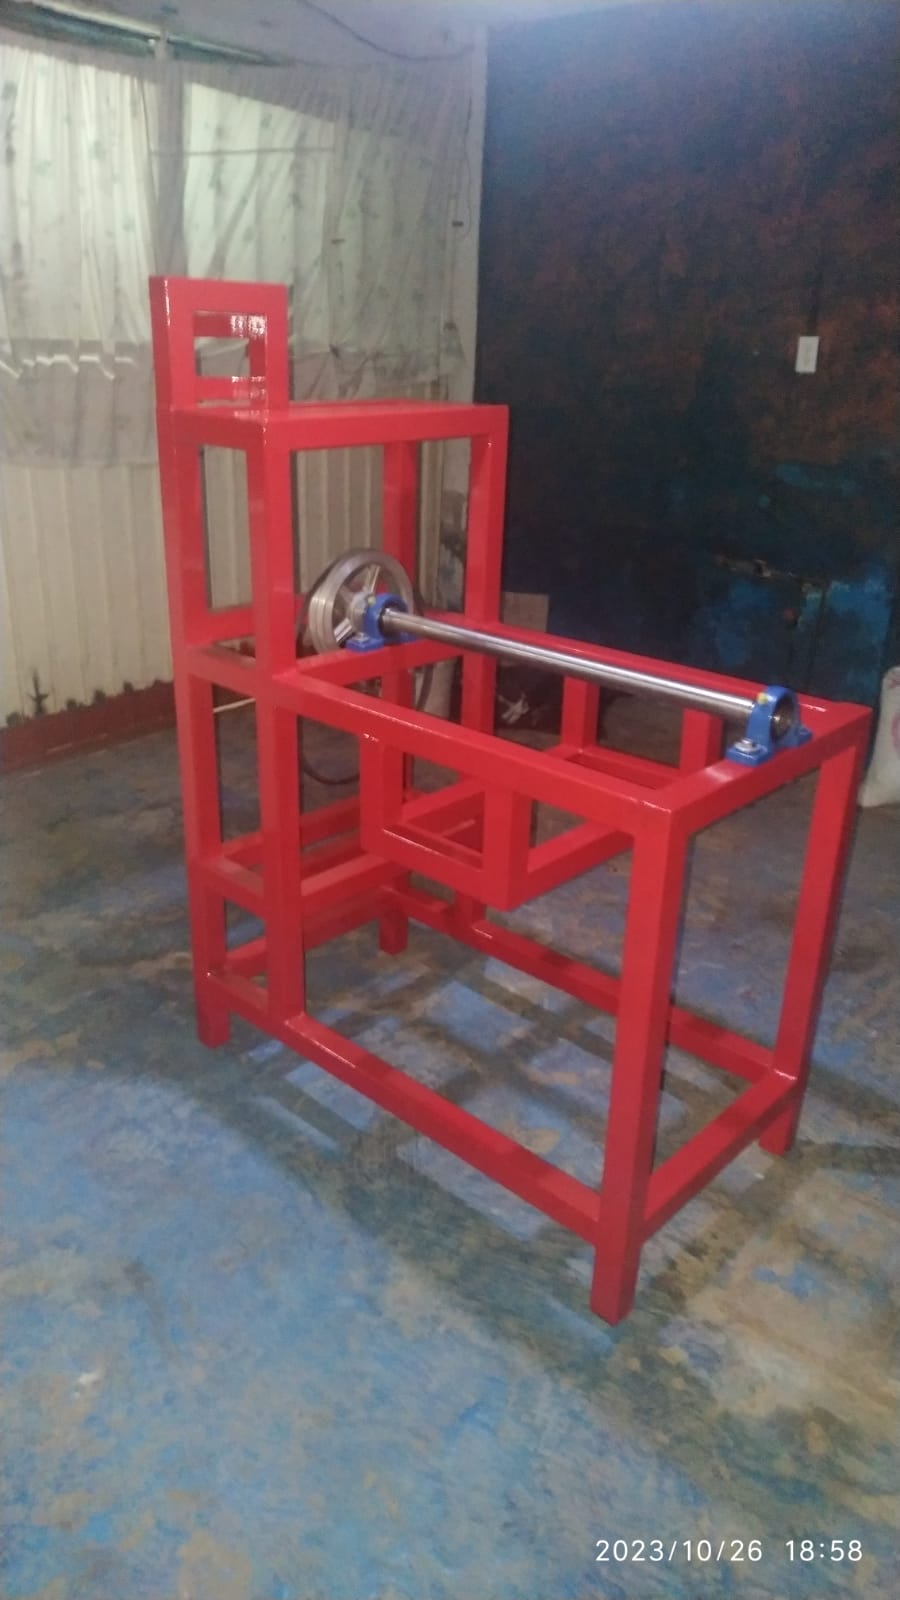
\includegraphics[scale=0.135]{images/Capitulo_Imple/S6/estructura.jpeg}
            \caption{Estructura del sistema de compostaje}
            \label{fg:estructura elaborada}
 \end{figure}

 \clearpage

